\newpage
% ==========================================
%              CHAPTER THREE
% ==========================================
\thispagestyle{plain}

\begin{center}
    \vspace*{0.5cm}
    {\large \textit{Chapter Three}} \\[0.4cm]
    {\Large \textbf{3 \quad METHODOLOGY --- LETTER RECOGNITION}}
\end{center}
\addcontentsline{toc}{chapter}{\textbf{3 \quad METHODOLOGY --- LETTER RECOGNITION}}
\vspace{1in}

\normalsize
\startchapterfloats{3}

\noindent Chapter~2 reviewed the literature and justified Eshara's design funnel (static MLP paradigm for letters; as set out in Table~\ref{tab:feature-vectors}, Chapter~2). This chapter specifies \emph{how} finger-spelling recognition is implemented: shared system architecture, letter datasets, MediaPipe Hands feature extraction, the two letter MLP pipelines, temporal stabilisation, Arabic UI rendering, engineering trade-offs, and evaluation protocol. Isolated \textbf{word} recognition methodology is presented in Chapter~4~\cite{akash2019aslalphabet,arthur2018arasl2018,zhang2020mediapipe}.\par\vspace{0.6cm}

% --- 3.1 ARCHITECTURE ---
\noindent\textbf{3.1\quad HIGH-LEVEL SYSTEM ARCHITECTURE}\par
\addcontentsline{toc}{section}{\numberline{3.1}HIGH-LEVEL SYSTEM ARCHITECTURE}
\vspace{0.4cm}

\noindent Eshara is a three-tier web application. The \textbf{browser} captures webcam frames and sends authenticated requests to a \textbf{Node.js/Express} API gateway; the gateway proxies inference requests internally to \textbf{FastAPI} model services over HTTP~\cite{rfc9110,fastapi,react}. The inference tier loads standalone checkpoints at startup --- letter MLPs and the ArSL word BiLSTM as Keras \texttt{.h5} files, the ASL word I3D as a PyTorch \texttt{.pt} file --- and returns JSON predictions. Letter models use no external scaler; the deployed ArSL word BiLSTM likewise consumes raw nose/wrist-centred coordinates without a saved \texttt{StandardScaler} (Chapter~4). The \textbf{React} UI renders letter streams (with a stability decoder) or isolated word labels, with RTL layout for Arabic text output~\cite{wcag22}.\par\vspace{0.4cm}

\noindent The runtime path for \textbf{letter} inference is:
\begin{enumerate}
\item User selects language (EN/AR) and \textbf{letter} mode in the React client.
\item The inference service runs MediaPipe \textbf{Hands} to extract 21 landmarks per frame and builds a language-specific feature vector (63-D raw for ArSL; 78-D engineered for ASL).
\item Each frame's vector is classified immediately by the language-specific letter MLP; a stabilisation decoder commits stable characters.
\item FastAPI routes the request to the correct model, returns \texttt{\{prediction, confidence, top\_k\}}, and the UI updates (with Arabic reshaping when ArSL is selected).
\end{enumerate}
\vspace{0.4cm}

\noindent This decomposition ensures (i)~\textbf{consistency} --- all users share the same server-side weights; (ii)~\textbf{security control} --- requests are validated and authenticated at the Node gateway; and (iii)~\textbf{modularity} --- each model can be retrained and redeployed independently~\cite{zhang2020mediapipe,rfc6455}.\par\vspace{0.4cm}

\noindent\textbf{Design invariant:} no shared vocabulary across models. ASL glosses do not align with ArSL glosses; letter and word label spaces differ even within one language. Four parallel classifiers behind one API enforce this constraint at deployment time.\par\vspace{0.4cm}

\noindent Word-mode buffering (32-frame RGB for ASL I3D; 48-frame Holistic for ArSL BiLSTM) is described in Chapter~4.\par\vspace{0.4cm}

\begin{figure}[H]
\centering
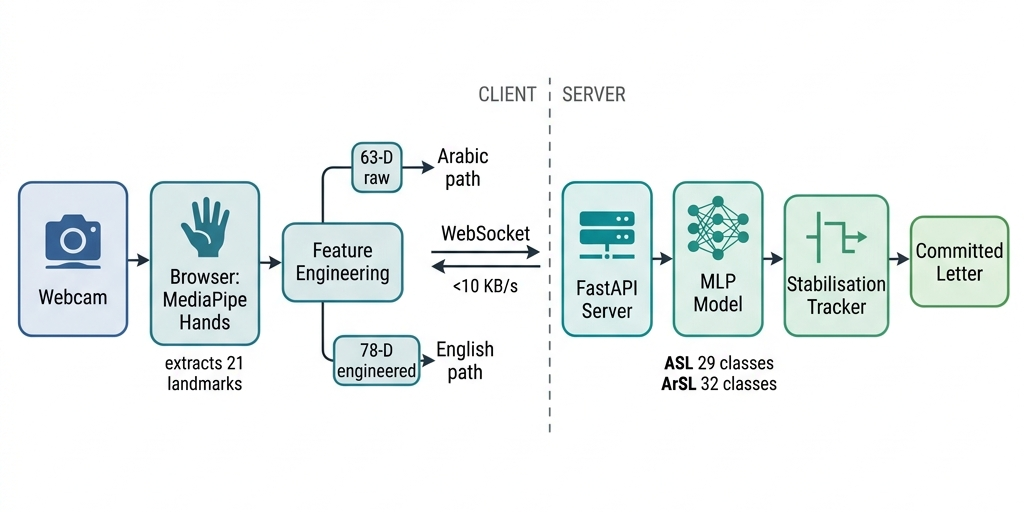
\includegraphics[width=0.90\textwidth]{images/fig_3-3_letter_pipeline.png}
\caption{Letter-mode client--server pipeline. The browser captures a webcam frame as a base64-encoded JPEG and sends it via HTTP \texttt{POST} to the Node.js application tier; the gateway proxies the request to FastAPI, where MediaPipe Hands extracts landmarks and engineers a 63-D (ArSL) or 78-D (ASL) vector before the letter MLP and stabilisation decoder commit a character.}
\label{fig:ch3-letter-pipeline}
\end{figure}
\vspace{0.6cm}
\clearpage
% --- 3.2 DATASETS ---
\noindent\textbf{3.2\quad LETTER DATASETS AND SPLIT POLICIES}\par
\addcontentsline{toc}{section}{\numberline{3.2}LETTER DATASETS AND SPLIT POLICIES}
\vspace{0.4cm}

\noindent The following table summarises the two letter corpora. Static images use random stratified splits~\cite{akash2019aslalphabet,arthur2018arasl2018}.\par\vspace{0.4cm}

\begin{table}[H]
\centering
\caption{Letter datasets, feature shapes, and split policies.}
\label{tab:ch3-letter-datasets}
\small
\begin{tabular}{|P{1.5cm}|P{2.2cm}|c|c|c|P{2.8cm}|}
\hline
\textbf{Task} & \textbf{Dataset} & \textbf{Classes} & \textbf{Features} & \textbf{Frames} & \textbf{Split} \\
\hline
ASL letters & ASL Alphabet & 29 (28 deploy.) & 78-D & 1 & $\sim$64/16/20 train/val/test \\
ArSL letters & ArASL2018 & 32 & 63-D & 1 & 60/20/20 train/val/test \\
\hline
\end{tabular}
\end{table}
\vspace{0.4cm}

\noindent\textbf{Training software environment.} Letter and word training share a common Python stack (as defined in Table~\ref{tab:ch3-env}). Heavy jobs --- Holistic extraction over KArSL videos and Inception I3D fine-tuning experiments --- were run on \textbf{Kaggle GPU} (T4/P100/L4, CUDA~11.x) when local VRAM was insufficient; letter MLP training and live prototyping used a \textbf{4\,GB NVIDIA GPU} on the development laptop. TensorFlow/Keras letter and ArSL word training enable GPU memory growth; PyTorch loads the ASL I3D checkpoint for server inference~\cite{abadi2016tensorflow,chollet2015keras,kingma2015adam}.\par\vspace{0.3cm}

\begin{table}[H]
\centering
\caption{Training and inference software environment (letters and words).}
\label{tab:ch3-env}
\small
\begin{tabular}{|l|l|}
\hline
\textbf{Component} & \textbf{Version / role} \\
\hline
Python & 3.9+ \\
TensorFlow / Keras~\cite{abadi2016tensorflow,chollet2015keras} & 2.x --- letter MLPs, ArSL word BiLSTM \\
PyTorch~\cite{pytorch2024} & 2.x --- ASL word Inception I3D (\texttt{asl\_word\_i3d.pt}) \\
CUDA / cuDNN~\cite{chetlur2014cudnn} & 11.x (Kaggle GPU; local 4\,GB GPU when available) \\
MediaPipe~\cite{zhang2020mediapipe,mediapipeweb} & 0.10.x (Python extraction; JS/WASM in browser) \\
OpenCV, NumPy, scikit-learn~\cite{opencv2024docs,harris2020numpy,pedregosa2011sklearn} & Feature I/O, metrics \\
Jupyter~\cite{kluyver2016jupyter} & Interactive training environment \\
Adam optimiser~\cite{kingma2015adam} & $\eta{=}10^{-3}$ default (letters); word schedules in Ch.~4 \\
\hline
\end{tabular}
\end{table}
\vspace{0.3cm}
\clearpage
\noindent\textbf{3.2.1\quad ASL Alphabet (English Letters):}\par
\addcontentsline{toc}{subsection}{\numberline{3.2.1}ASL Alphabet (English Letters):}
\vspace{0.3cm}
\noindent The Kaggle ASL Alphabet corpus provides $\sim$87\,000 static hand images across 29 classes (A--Z plus \texttt{space}, \texttt{del}, \texttt{nothing})~\cite{akash2019aslalphabet}. The graduation \textbf{deployed} ASL letter model excludes the \texttt{nothing} control class, yielding a 28-way label space (Chapter~6). Images are converted \textbf{offline} to MediaPipe Hand landmarks, then augmented with wrist-relative normalisation and 15 inter-joint angles to form a 78-D engineered vector cached in CSV/NPZ before MLP training. The \textbf{same} 78-D representation is computed in the browser at inference time, eliminating train/serve skew on input geometry~\cite{zhang2020mediapipe}.\par\vspace{0.4cm}

\noindent\textbf{3.2.2\quad ArASL2018 (Arabic Letters):}\par
\addcontentsline{toc}{subsection}{\numberline{3.2.2}ArASL2018 (Arabic Letters):}
\vspace{0.3cm}

\noindent ArASL2018 provides 54\,049 images across 32 Arabic finger-spelling classes~\cite{arthur2018arasl2018}. Processing mirrors the landmark extraction stage of the ASL pipeline but uses the flattened 63-D raw coordinate vector without additional angle features. Visually similar letter pairs (e.g.\ \arTxt{ك}/\arTxt{ل}) motivate per-class evaluation in Chapter~6. Model~2 shares the same \textbf{MLP family} as Model~1 (Dense--BN--ReLU--Dropout blocks) but uses a \textbf{wider, separately trained head} with different input dimension, hidden widths, and hyperparameters (Section~3.5; Table~\ref{tab:ch3-arch-compare}).\par\vspace{0.4cm}

\noindent\textbf{3.2.3\quad End-to-End Training Pipeline (Dataset to \texttt{.h5} Artifact):}\par
\addcontentsline{toc}{subsection}{\numberline{3.2.3}End-to-End Training Pipeline:}
\vspace{0.3cm}

\noindent Both letter corpora follow the same offline preparation and training pipeline. The numbered steps below trace the complete path from raw image dataset to the exported checkpoint used by the FastAPI inference service.

\begin{enumerate}

\item \textbf{Image loading.} Dataset images are read from disk (JPEG/PNG) and converted to RGB. MediaPipe Hands is initialised with \texttt{static\_image\_mode=True}, \texttt{max\_num\_hands=1}, and \texttt{min\_detection\_confidence=0.7}. Unreadable or empty files are skipped.

\item \textbf{Landmark extraction.} For each image, MediaPipe returns 21 hand landmarks $\{(x_i, y_i, z_i)\}_{i=0}^{20}$ normalised to image coordinates $[0,1]^2$ with depth estimate $z_i$. Images where no hand is detected are discarded. Detection rates are approximately 69\,\% for ASL Alphabet and 77\,\% for ArASL2018, yielding $\sim$60\,k and $\sim$74\,k successful samples respectively.

\item \textbf{Feature engineering.} Extracted landmarks are transformed into a fixed-length feature vector (see Section~3.3):
\[
\mathbf{x} = \begin{cases} \mathbf{x}_{\text{raw}} \in \mathbb{R}^{63} & \text{ArSL: flatten } (x_i, y_i, z_i)^\top \text{ directly,} \\ \mathbf{x}_{\text{ASL}} \in \mathbb{R}^{78} & \text{ASL: wrist-centred 21 landmarks + 15 angles ($63{+}15$).}\end{cases}
\]

\item \textbf{Caching.} Feature vectors and class labels are written to a CSV file (\texttt{asl\_letters\_engineered.csv} / \texttt{ASLAD-3000\_v2.csv}) and a compressed NPZ archive for fast NumPy loading. This step runs once; subsequent training passes load directly from cache.

\item \textbf{Train / validation / test split.} The feature matrix $X \in \mathbb{R}^{N \times d}$ is split with \textbf{stratified} sampling (preserving per-class proportions) using \texttt{random\_state=42}:
\begin{equation}
\label{eq:ch3-split}
(X_{\text{train}},\, X_{\text{val}},\, X_{\text{test}}) \quad \text{proportions } \begin{cases} 0.64 : 0.16 : 0.20 & \text{(ASL)} \\ 0.60 : 0.20 : 0.20 & \text{(ArSL)} \end{cases}
\end{equation}
Test split is isolated before any hyperparameter search and is touched exactly once for final reporting.

\item \textbf{One-hot label encoding.} Integer class indices are converted to one-hot vectors:
\begin{equation}
\label{eq:ch3-onehot}
\mathbf{y} = \mathbf{e}_c \in \{0,1\}^C, \qquad e_{c,k} = \mathbb{1}[k = c], \qquad C \in \{28,\,32\},
\end{equation}
via Keras \texttt{to\_categorical} (or \texttt{np.eye} for ArSL when TensorFlow is loaded later in the pipeline). Feature vectors are fed \textbf{directly} to the MLP without an external \texttt{StandardScaler}; batch normalisation inside the network handles activation scaling during training. (Deployed word models likewise use no external scaler at inference; see Chapter~4.)

\item \textbf{Model construction.} The MLP is assembled with the Keras \texttt{Sequential} API. Layer widths, BN placement, dropout rates, and output softmax dimension are specified per model (Sections~3.4 and~3.5; Figure~\ref{fig:ch3-mlp-heads}).

\item \textbf{Callbacks.} Three callbacks are registered before \texttt{model.fit}:
\begin{itemize}
  \item \textbf{ModelCheckpoint}~\cite{chollet2015keras}: saves the \texttt{.h5} artifact to disk whenever \texttt{val\_accuracy} improves (\texttt{save\_best\_only=True}, \texttt{mode='max'}).
  \item \textbf{EarlyStopping}~\cite{chollet2015keras}: monitors \texttt{val\_loss}; halts training when no improvement is seen for \texttt{patience} consecutive epochs and restores the best weights (\texttt{restore\_best\_weights=True}).
  \item \textbf{ReduceLROnPlateau} (ArSL only)~\cite{chollet2015keras}: multiplies the current learning rate by factor 0.5 when \texttt{val\_loss} does not improve for 7 consecutive epochs, floored at $\eta_{\min} = 10^{-7}$.
\end{itemize}

\item \textbf{Mini-batch training.} Parameters $\theta$ are updated over mini-batches of size $B \in \{64,\,256\}$ using the Adam optimiser. At each step $t$ with gradient $g_t = \nabla_\theta \mathcal{L}$:
\begin{align}
m_t &= \beta_1 m_{t-1} + (1-\beta_1)\, g_t, \label{eq:adam-m}\\
v_t &= \beta_2 v_{t-1} + (1-\beta_2)\, g_t^2, \label{eq:adam-v}\\
\hat{m}_t &= \frac{m_t}{1-\beta_1^t}, \qquad \hat{v}_t = \frac{v_t}{1-\beta_2^t}, \label{eq:adam-bias}\\
\theta_t &\leftarrow \theta_{t-1} - \eta\,\frac{\hat{m}_t}{\sqrt{\hat{v}_t}+\varepsilon_A}, \label{eq:adam-update}
\end{align}
with defaults $\beta_1{=}0.9$, $\beta_2{=}0.999$, $\varepsilon_A{=}10^{-7}$~\cite{kingma2015adam}.

\item \textbf{Test evaluation.} After training, the best checkpoint is loaded and evaluated \textbf{once} on the held-out test split. Top-1 accuracy, test loss, and a per-class classification report (precision, recall, F1) are recorded for Chapter~6.

\item \textbf{Artifact export.} The best \texttt{.h5} checkpoint is the final deliverable:
\begin{itemize}
  \item ASL: \texttt{asl\_mediapipe\_mlp\_model\_engineered.h5}
  \item ArSL: \texttt{arsl\_mediapipe\_mlp\_model\_bestV2.2.h5}
\end{itemize}
The FastAPI inference service loads these at startup (Chapter~5); no further post-processing (quantisation, pruning) is applied within graduation scope.

\end{enumerate}
\vspace{0.4cm}

\noindent The complete workflow is illustrated in the following figure after the feature definitions in Section~3.3.\par\vspace{0.4cm}

% --- 3.3 FEATURES ---
\noindent\textbf{3.3\quad FEATURE EXTRACTION FOR LETTERS}\par
\addcontentsline{toc}{section}{\numberline{3.3}FEATURE EXTRACTION FOR LETTERS}
\vspace{0.4cm}

\noindent MediaPipe Hands outputs 21 $(x,y,z)$ points per hand~\cite{zhang2020mediapipe}. For finger-spelling, \texttt{max\_num\_hands=1} suffices; face and pose modules are reserved for word models (Chapter~4). Missing landmarks are zero-filled; the live client mirrors training conventions. As shown in Figure~\ref{fig:ch3-landmarks}, the diagram labels the wrist (0) and the four finger chains (thumb 1--4, index 5--8, middle 9--12, ring 13--16, pinky 17--20).\par\vspace{0.4cm}

\begin{figure}[H]
\centering
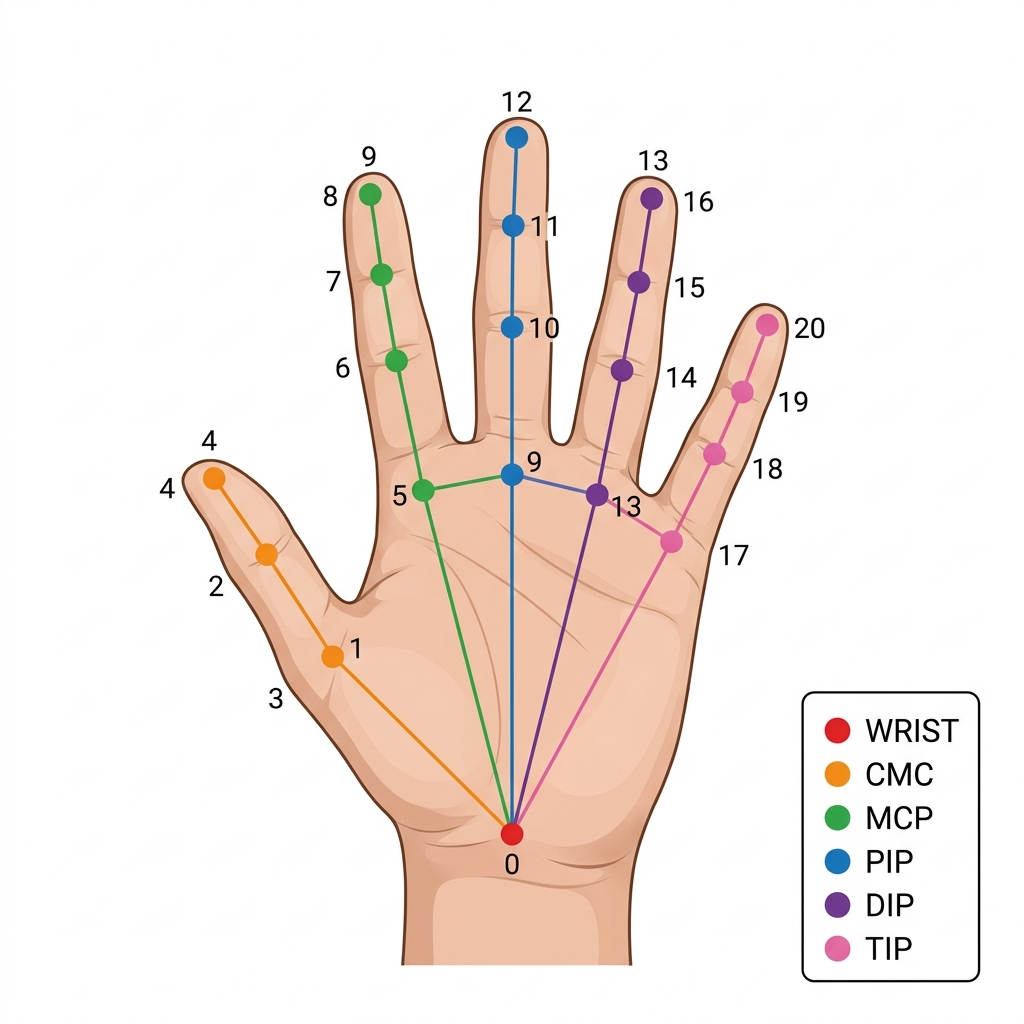
\includegraphics[width=0.9\textwidth]{images/fig_3-1_mediapipe_landmarks.png}
\caption{MediaPipe Hand landmark topology (21 points). Each landmark contributes $(x,y,z)$ coordinates; flattening yields a 63-D raw vector.}
\label{fig:ch3-landmarks}
\end{figure}
\vspace{0.4cm}

\begin{figure}[H]
\centering
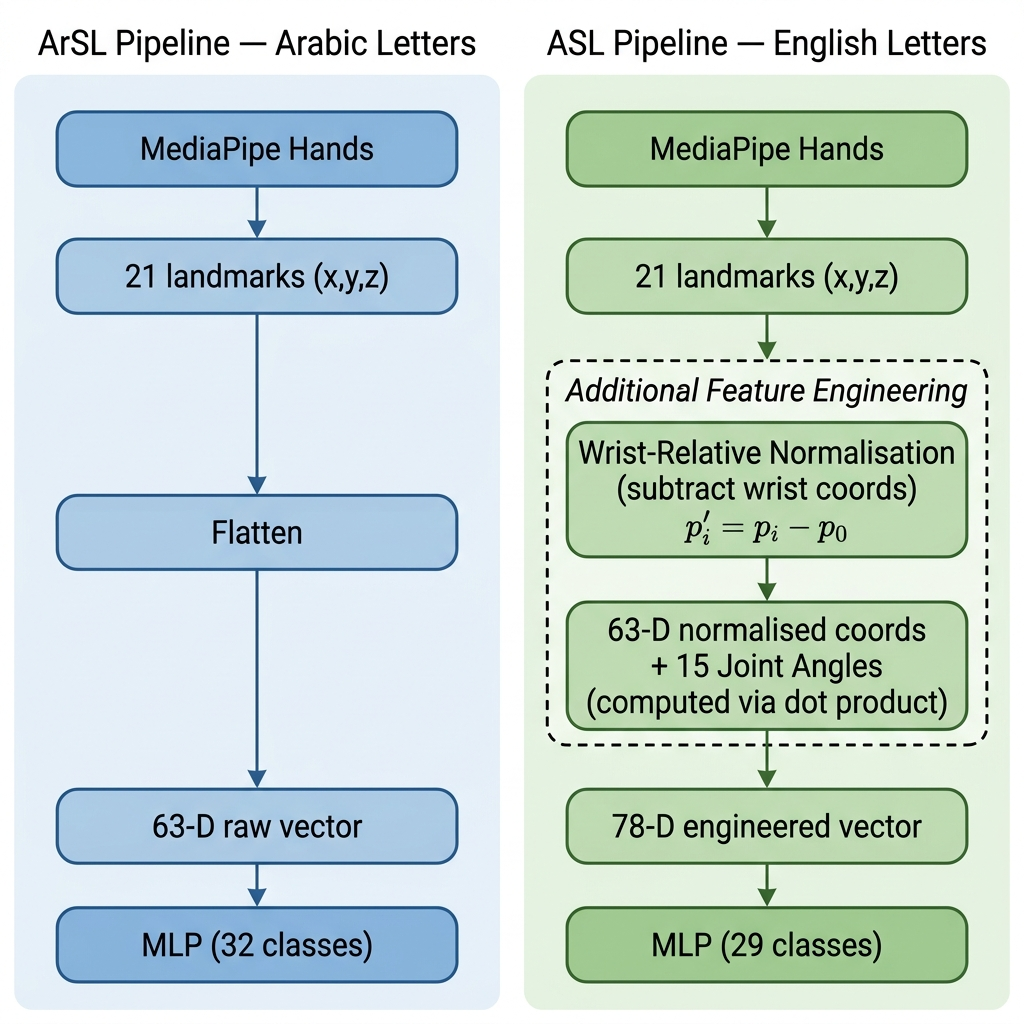
\includegraphics[width=0.88\textwidth]{images/fig_3-5_feature_engineering.png}
\caption{Letter feature-engineering split. ArSL (left): MediaPipe Hands $\rightarrow$ flatten $\rightarrow$ 63-D raw MLP (32 classes). ASL (right): additional wrist-relative normalisation and 15 joint angles $\rightarrow$ 78-D engineered MLP (28 deployed classes).}
\label{fig:ch3-feature-eng}
\end{figure}
\vspace{0.4cm}

\noindent The two letter pipelines diverge after landmark extraction (as illustrated in Figure~\ref{fig:ch3-feature-eng}). Let $\mathbf{p}_i = (x_i, y_i, z_i)^\top \in \mathbb{R}^3$ denote landmark $i$ with wrist index $i{=}0$. The raw feature vector is
\begin{equation}
\label{eq:ch3-x-raw}
\mathbf{x}_{\text{raw}} = \bigl[x_0, y_0, z_0, x_1, y_1, z_1, \ldots, x_{20}, y_{20}, z_{20}\bigr]^\top \in \mathbb{R}^{63}.
\end{equation}
\textbf{ArSL (Model~2)} uses $\mathbf{x}_{\text{raw}}$ directly. \textbf{ASL (Model~1)} wrist-centres every landmark and appends 15 inter-joint angles:
\begin{equation}
\mathbf{p}'_i = \mathbf{p}_i - \mathbf{p}_0, \qquad i = 0,\ldots,20,
\end{equation}
\begin{equation}
\theta_j = \arccos\!\left(\frac{\mathbf{v}_{j,1} \cdot \mathbf{v}_{j,2}}{\|\mathbf{v}_{j,1}\|\,\|\mathbf{v}_{j,2}\| + \epsilon}\right), \qquad j = 1,\ldots,15,
\end{equation}
where $\mathbf{v}_{j,1} = \mathbf{p}'_{a_j} - \mathbf{p}'_{b_j}$ and $\mathbf{v}_{j,2} = \mathbf{p}'_{c_j} - \mathbf{p}'_{b_j}$ are the two bone vectors meeting at joint $b_j$ (the middle landmark of the triplet $(a_j, b_j, c_j)$), and $\epsilon{=}10^{-8}$ avoids division by zero. The 15 triplets cover three joints per finger (metacarpo-phalangeal MCP, proximal inter-phalangeal PIP, distal inter-phalangeal DIP) across all five fingers, as defined in Table~\ref{tab:ch3-angle-triplets}. The deployed ASL input concatenates all wrist-centred coordinates with the angle block:
\begin{equation}
\label{eq:ch3-x-asl}
\mathbf{x}_{\text{ASL}} = \bigl[\,\mathbf{p}'_0, \ldots, \mathbf{p}'_{20};\; \theta_1, \ldots, \theta_{15}\,\bigr]^\top \in \mathbb{R}^{78},
\end{equation}
i.e.\ $21 \times 3 = 63$ translation-invariant landmark values (with $\mathbf{p}'_0 \equiv \mathbf{0}$) plus 15 scalar angles. The same 78-D layout is reproduced in the browser at inference time~\cite{zhang2020mediapipe}.

\begin{table}[H]
\centering
\caption{The 15 inter-joint angle triplets used in the 78-D ASL feature vector. Each row specifies the landmark index triple $(a, b, c)$ where $b$ is the vertex joint; the angle is computed between bone vectors $b{\to}a$ and $b{\to}c$.}
\label{tab:ch3-angle-triplets}
\small
\begin{tabular}{|l|c|c|}
\hline
\textbf{Finger} & \textbf{Joint} & \textbf{Triplet $(a, b, c)$} \\
\hline
Thumb  & MCP & (0, 1, 2) \\
Thumb  & PIP & (1, 2, 3) \\
Thumb  & DIP & (2, 3, 4) \\
Index  & MCP & (0, 5, 6) \\
Index  & PIP & (5, 6, 7) \\
Index  & DIP & (6, 7, 8) \\
Middle & MCP & (0, 9, 10) \\
Middle & PIP & (9, 10, 11) \\
Middle & DIP & (10, 11, 12) \\
Ring   & MCP & (0, 13, 14) \\
Ring   & PIP & (13, 14, 15) \\
Ring   & DIP & (14, 15, 16) \\
Pinky  & MCP & (0, 17, 18) \\
Pinky  & PIP & (17, 18, 19) \\
Pinky  & DIP & (18, 19, 20) \\
\hline
\end{tabular}
\end{table}
\vspace{0.4cm}

\noindent The following table summarises the complete feature-vector composition for each letter model, cross-referencing dimensions to the equations above.

\begin{table}[H]
\centering
\caption{Feature-vector dimension breakdown for the two letter models.}
\label{tab:ch3-feature-dim}
\small
\begin{tabular}{|P{2.4cm}|r|P{3.6cm}|P{3.6cm}|}
\hline
\textbf{Component} & \textbf{Dims} & \textbf{ASL (Model~1)} & \textbf{ArSL (Model~2)} \\
\hline
Wrist-centred coords $\mathbf{p}'_{0\ldots20}$ & 63 & Yes (Eq.~\eqref{eq:ch3-x-asl}) & No (raw wrist incl.) \\
Raw wrist $(x_0,y_0,z_0)$                        &  3 & (included in $\mathbf{p}'_0{=}\mathbf{0}$) & Yes \\
Raw landmarks $\mathbf{p}_{1\ldots20}$           & 60 & No  & Yes \\
Joint angles $\theta_{1\ldots15}$                & 15 & Yes (Table~\ref{tab:ch3-angle-triplets}) & No \\
\hline
\textbf{Total}                                   & \textbf{78} / \textbf{63} & \textbf{78-D} & \textbf{63-D} \\
\hline
\end{tabular}
\end{table}
\vspace{0.4cm}

\noindent Holistic/Pose+Hands extensions for word models are summarised as set out in Table~\ref{tab:feature-vectors} (Chapter~2).\par\vspace{0.4cm}

\noindent As summarised in Figure~\ref{fig:ch3-training-pipeline}, the offline training path runs from dataset images to the exported \texttt{.h5} checkpoint. Shared stages (landmark extraction through label encoding) are identical for both languages; ASL and ArSL diverge at feature engineering and at MLP head configuration (as compared in Figure~\ref{fig:ch3-mlp-heads} and Table~\ref{tab:ch3-arch-compare}).

\begin{figure}[H]
\centering
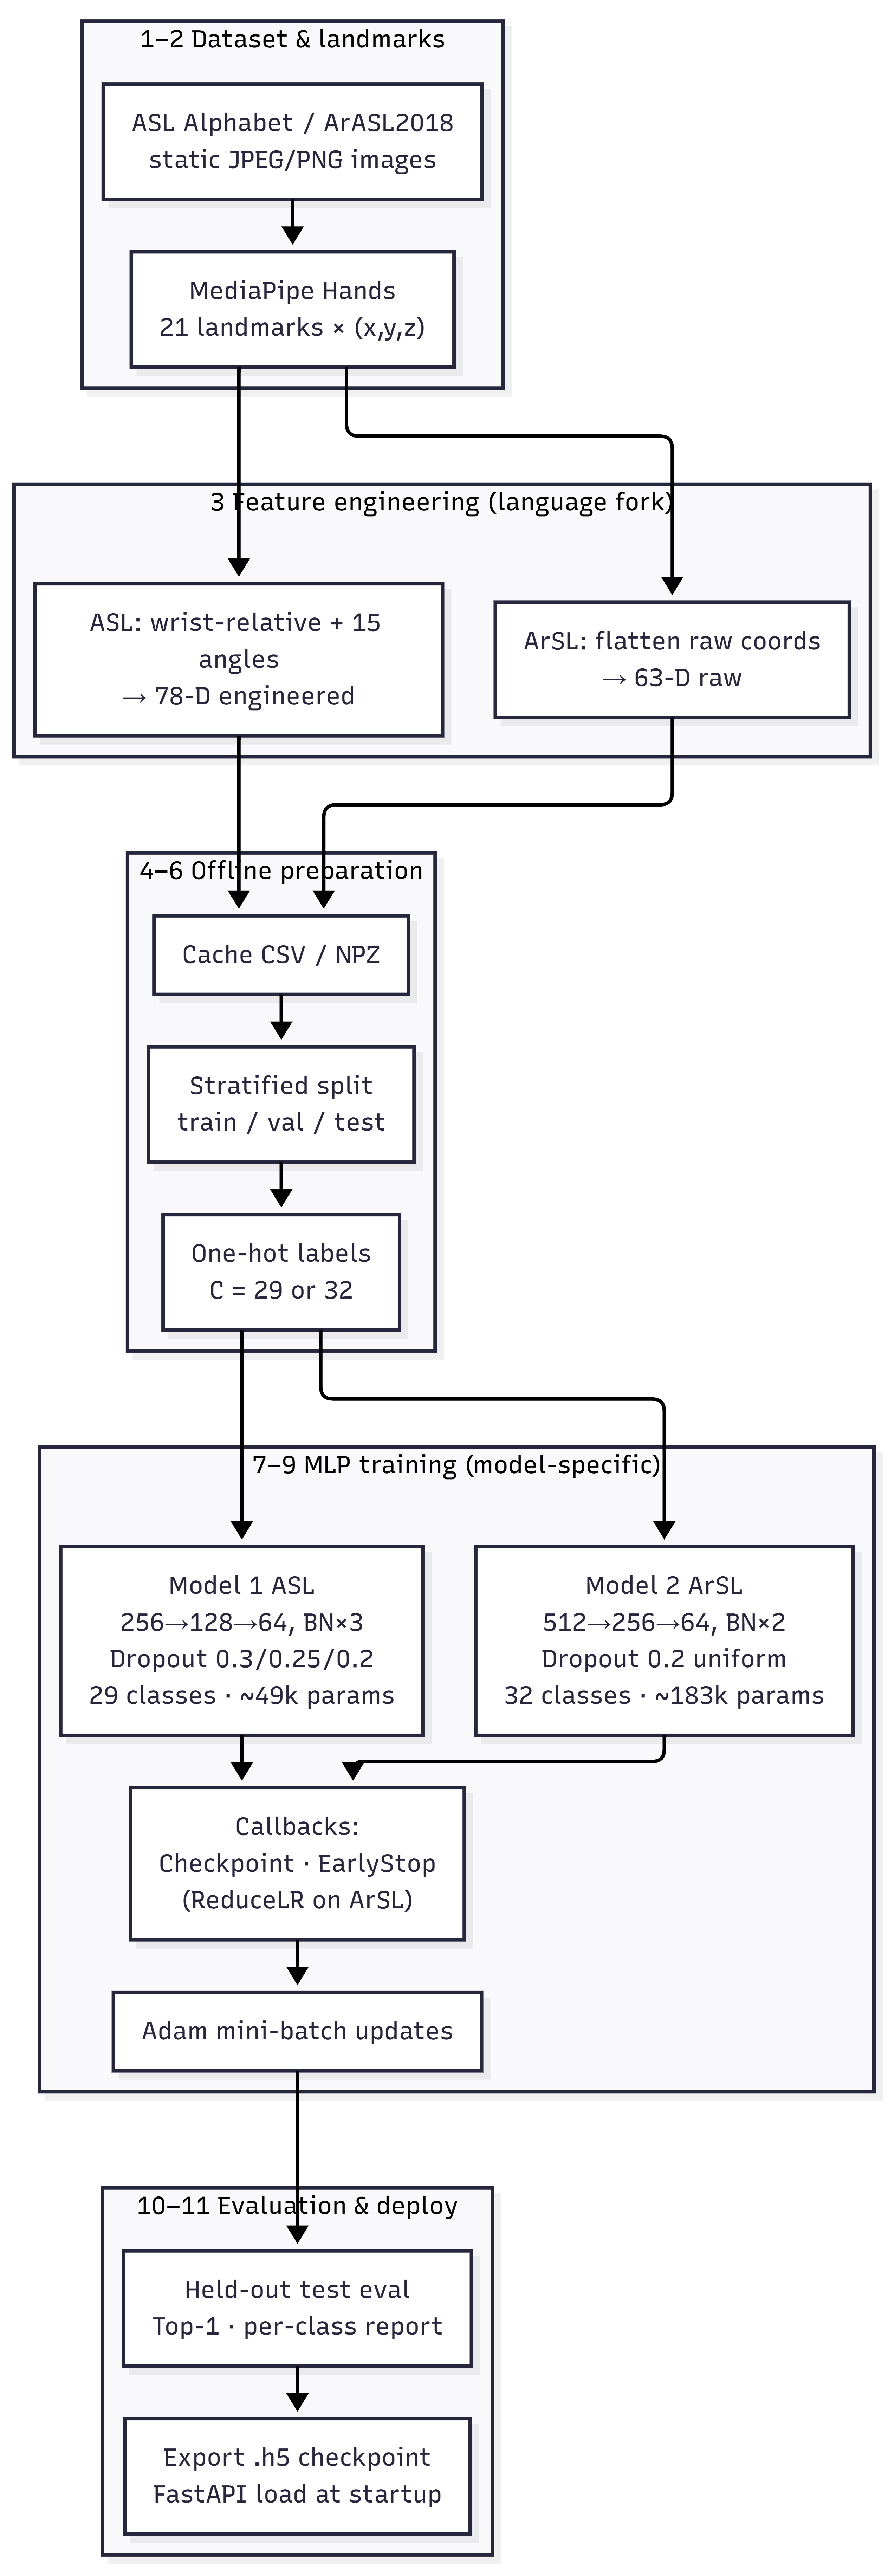
\includegraphics[width=0.90\textwidth,height=0.95\textheight,keepaspectratio]{images/fig_3-8_letter_training_pipeline.png}
\caption{End-to-end letter training pipeline. Stages~1--6 are shared; language-specific forks appear at feature engineering (78-D engineered vs.\ 63-D raw) and at MLP head width, dropout, and training schedule.}
\label{fig:ch3-training-pipeline}
\end{figure}
\vspace{0.6cm}

% --- 3.4 MODEL 1 ---
\noindent\textbf{3.4\quad MODEL 1 --- ASL LETTER MLP}\par
\addcontentsline{toc}{section}{\numberline{3.4}MODEL 1 --- ASL LETTER MLP}
\vspace{0.15cm} % Cramped from 0.4cm

\noindent\textbf{Problem:} finger-spelled ASL letters are quasi-static poses; one frame suffices~\cite{akash2019aslalphabet}.\par\vspace{0.15cm} % Cramped from 0.3cm

\noindent\textbf{Input and notation.} Each training or inference sample is a single engineered vector $\mathbf{x} \in \mathbb{R}^{78}$ from Equation~\eqref{eq:ch3-x-asl}. The model implements a three-hidden-layer MLP with batch normalisation, ReLU, dropout, and softmax (Figures~\ref{fig:ch3-mlp} and~\ref{fig:ch3-mlp-heads}). Layer widths are $d_0{=}78$, $d_1{=}256$, $d_2{=}128$, $d_3{=}64$, and output dimension $C{=}28$ (A--Z, \texttt{space}, \texttt{del}).\par\vspace{0.15cm} % Cramped from 0.3cm

% --- MATH SPACING OVERRIDE ---
% This block temporarily shrinks the massive empty spaces LaTeX puts around equations
\begingroup
\setlength{\abovedisplayskip}{3pt}
\setlength{\belowdisplayskip}{3pt}
\setlength{\abovedisplayshortskip}{3pt}
\setlength{\belowdisplayshortskip}{3pt}

\noindent\textbf{Forward pass.} Each hidden block $\ell \in \{1,2,3\}$ applies a dense affine transform, batch normalisation, ReLU, and dropout (Section~2.4.1 summarises the MLP family at a high level). With input $\mathbf{h}^{(0)} = \mathbf{x}$, layer $\ell$ computes
\begin{equation}
\tilde{\mathbf{h}}^{(\ell)} = W^{(\ell)} \mathbf{h}^{(\ell-1)} + \mathbf{b}^{(\ell)}, \qquad \mathbf{h}^{(\ell)} = \mathrm{Dropout}_p\!\Big(\mathrm{ReLU}\big(\mathrm{BN}(\tilde{\mathbf{h}}^{(\ell)})\big)\Big),
\end{equation}
with $\mathbf{h}^{(0)} = \mathbf{x}$. Batch normalisation~\cite{ioffe2015batchnorm} standardises each pre-activation batch dimension:
\begin{equation}
\mathrm{BN}(\tilde{h}) = \gamma \,\frac{\tilde{h} - \mu_B}{\sqrt{\sigma_B^2 + \epsilon}} + \beta,
\end{equation}
where $\mu_B$ and $\sigma_B^2$ are batch mean and variance at training time (running statistics at inference). Dropout~\cite{srivastava2014dropout} zeroes each activation independently with probability $p \in \{0.3, 0.25, 0.2\}$ on layers 1--3 respectively. Class logits $\mathbf{z} \in \mathbb{R}^{28}$ and probabilities follow
\begin{equation}
\mathbf{z} = W^{(4)} \mathbf{h}^{(3)} + \mathbf{b}^{(4)}, \qquad
P(y{=}k \mid \mathbf{x}) = \frac{\exp(z_k)}{\sum_{j=1}^{28} \exp(z_j)}.
\end{equation}
The predicted letter is $\hat{y} = \arg\max_k P(y{=}k \mid \mathbf{x})$.\par\vspace{0.15cm} % Cramped from 0.3cm

\noindent\textbf{Loss and optimisation.} Training minimises categorical cross-entropy over one-hot labels $\mathbf{y}$:
\begin{equation}
\mathcal{L}_{\text{CE}} = -\sum_{k=1}^{28} y_k \log P(y{=}k \mid \mathbf{x}).
\end{equation}
\endgroup % Ends the math spacing override
% -----------------------------

\enlargethispage{\baselineskip} % MAGIC TRICK: Forces this specific page to stretch one line longer at the bottom margin to catch the spilling text

\noindent Parameters are updated with the \textbf{Adam} optimiser~\cite{kingma2015adam} at $\eta{=}10^{-3}$. Adam maintains per-parameter first and second moment estimates $(m_t, v_t)$ with bias-correction; the update at step $t$ is identical in form to Equations~\eqref{eq:adam-m}--\eqref{eq:adam-update} in Section~3.2.3 with $\beta_1{=}0.9$, $\beta_2{=}0.999$, $\varepsilon_A{=}10^{-7}$. \textbf{EarlyStopping} halts training when \texttt{val\_loss} fails to decrease for \textbf{patience~=~5} consecutive epochs; \texttt{restore\_best\_weights=True} reloads the checkpoint that achieved the lowest validation loss. Maximum training duration is 20 epochs; ModelCheckpoint saves the best \texttt{val\_accuracy} snapshot as the exported artifact.\par\vspace{0.2cm} % Cramped from 0.3cm

\clearpage

\noindent\textbf{Parameter count.} The trainable weight count is approximately
\begingroup
\setlength{\abovedisplayskip}{3pt}
\setlength{\belowdisplayskip}{3pt}
\begin{equation}
|\theta| \approx \underbrace{78{\times}256 + 256}_{\text{layer 1}} + \underbrace{256{\times}128 + 128}_{\text{layer 2}} + \underbrace{128{\times}64 + 64}_{\text{layer 3}} + \underbrace{64{\times}28 + 28}_{\text{softmax}} \approx 49\text{k},
\end{equation}
\endgroup
excluding batch-norm scale/shift terms ($\sim$1.8\,k additional). This footprint supports sub-50\,ms single-frame inference on laptop CPU/GPU~\cite{zhang2020mediapipe}.\par\vspace{0.2cm} % Cramped from 0.3cm

\noindent\textbf{Training setup.} Batch size 256 (GPU) or 64 (CPU); exported artifact \texttt{asl\_\allowbreak mediapipe\_\allowbreak mlp\_\allowbreak model\_\allowbreak engineered.h5}.\par\vspace{0.3cm} % Cramped from 0.4cm

\begin{figure}[H]
\centering
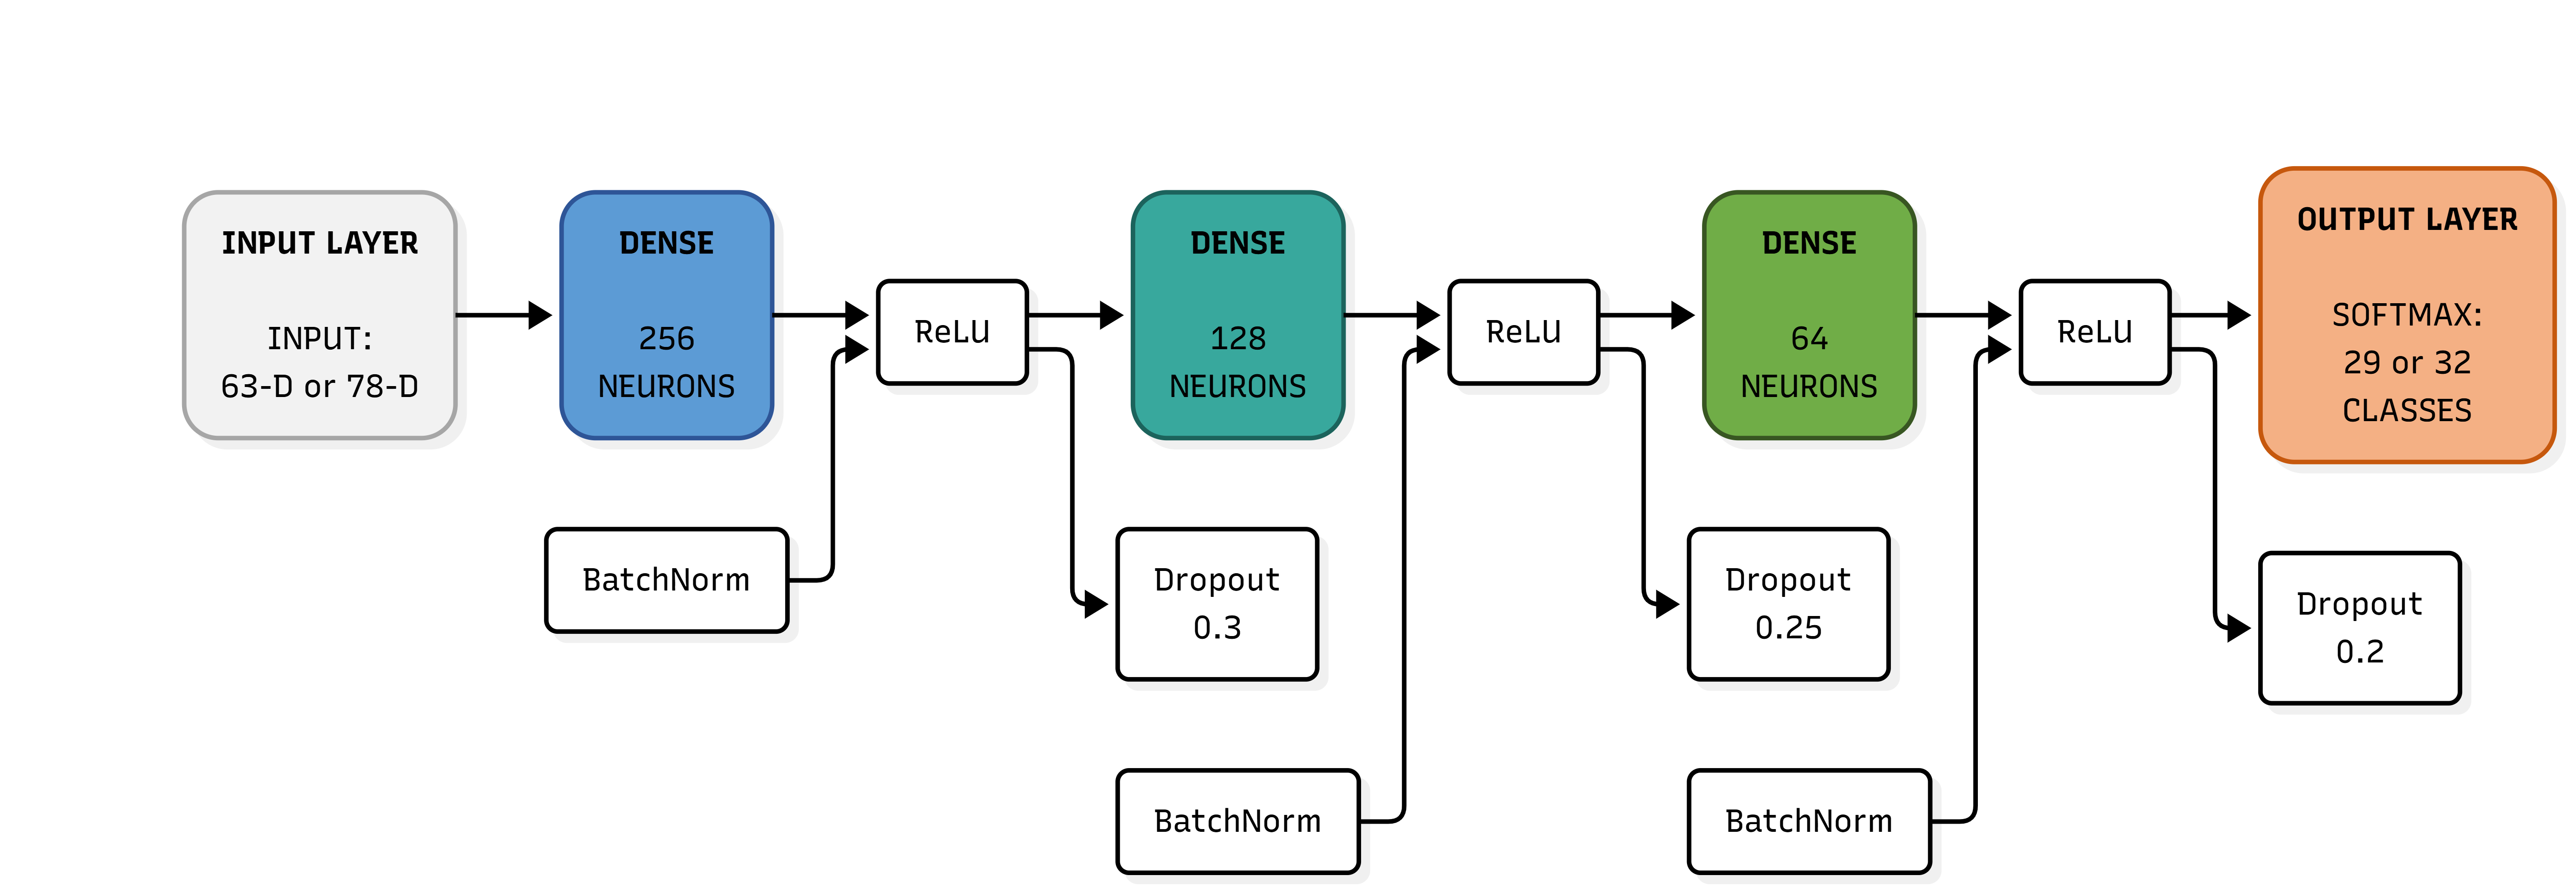
\includegraphics[width=0.9\textwidth]{images/fig_3-2_mlp_architecture.png}
\caption{Shared MLP \emph{family} for both letter models (Dense--BN--ReLU--Dropout--Softmax). ASL Model~1 uses 78-D input, widths 256/128/64, BN on all three hidden layers, and progressive dropout (0.3 / 0.25 / 0.2). ArSL Model~2 uses 63-D input, wider layers 512/256/64, BN on layers~1--2 only, and uniform dropout 0.2 (Table~\ref{tab:ch3-arch-compare}).}
\label{fig:ch3-mlp}
\end{figure}
\vspace{0.4cm} % Cramped from 0.6cm

% --- 3.5 MODEL 2 ---
\noindent\textbf{3.5\quad MODEL 2 --- ArSL LETTER MLP}\par
\addcontentsline{toc}{section}{\numberline{3.5}MODEL 2 --- ArSL LETTER MLP}
\vspace{0.4cm}

\noindent Model~2 shares the same \textbf{MLP family} as Model~1 but uses a wider architecture tuned on the ArSL corpus: input $\mathbf{x} \in \mathbb{R}^{63}$ equals $\mathbf{x}_{\text{raw}}$ from Equation~\eqref{eq:ch3-x-raw}; hidden widths are $d_1{=}512$, $d_2{=}256$, $d_3{=}64$ with uniform dropout $p{=}0.2$ on all three layers and batch normalisation after dense layers 1 and 2 only.\par\vspace{0.3cm}

\noindent\textbf{Forward pass.} Substituting $d_0{=}63$ into the Model~1 recurrence,
\begin{equation}
\mathbf{h}^{(0)} = \mathbf{x}_{\text{raw}}, \qquad
\tilde{\mathbf{h}}^{(\ell)} = W^{(\ell)} \mathbf{h}^{(\ell-1)} + \mathbf{b}^{(\ell)}, \quad \ell \in \{1,2,3\},
\end{equation}
with $W^{(1)} \in \mathbb{R}^{512 \times 63}$, $W^{(2)} \in \mathbb{R}^{256 \times 512}$, $W^{(3)} \in \mathbb{R}^{64 \times 256}$, and output weights $W^{(4)} \in \mathbb{R}^{32 \times 64}$. BN--ReLU--Dropout is applied after layers~1 and~2; layer~3 uses ReLU--Dropout (no BN). Class logits and probabilities are
\begin{equation}
\mathbf{z} = W^{(4)} \mathbf{h}^{(3)} + \mathbf{b}^{(4)}, \qquad
P(y{=}k \mid \mathbf{x}) = \frac{\exp(z_k)}{\sum_{j=1}^{32} \exp(z_j)}, \qquad \hat{y} = \arg\max_k P(y{=}k \mid \mathbf{x}).
\end{equation}
Training minimises the 32-way cross-entropy $\mathcal{L}_{\text{CE}} = -\sum_{k=1}^{32} y_k \log P(y{=}k \mid \mathbf{x})$ with Adam at $\eta_0{=}5\times10^{-4}$ (Equations~\eqref{eq:adam-m}--\eqref{eq:adam-update}). EarlyStopping monitors \texttt{val\_loss} with patience~15 and \texttt{restore\_best\_weights=True}; maximum epochs~100. ReduceLROnPlateau applies the schedule
\begin{equation}
\label{eq:rlrop}
\eta \leftarrow \max\!\bigl(\eta \times 0.5,\; \eta_{\min}\bigr), \qquad \eta_{\min} = 10^{-7},
\end{equation}
whenever \texttt{val\_loss} does not decrease for 7 consecutive epochs~\cite{kingma2015adam}. Mixed-precision training (\texttt{mixed\_float16}) is enabled on GPU, reducing memory by $\sim$50\,\%; the output dense layer is cast to \texttt{float32} to preserve softmax numerical stability.\par\vspace{0.3cm}

\noindent\textbf{Parameter count.} With $d_0{=}63$, $d_1{=}512$, $d_2{=}256$, $d_3{=}64$, and $C{=}32$,
\begin{equation}
|\theta| \approx \underbrace{63{\times}512 + 512}_{\text{layer 1}} + \underbrace{512{\times}256 + 256}_{\text{layer 2}} + \underbrace{256{\times}64 + 64}_{\text{layer 3}} + \underbrace{64{\times}32 + 32}_{\text{softmax}} \approx 183\text{k},
\end{equation}
excluding batch-norm scale/shift terms ($\sim$1.5\,k). Model~2 is wider than Model~1 to compensate for the higher intra-class variation and visually similar letter pairs in the ArSL corpus. \textbf{No weight sharing} with Model~1 --- ASL and ArSL finger-spelling use disjoint vocabularies and feature spaces~\cite{arthur2018arasl2018}. Raw coordinates suffice for ArASL2018 because wrist position is already consistent in the studio-captured corpus; ASL benefits from explicit translation and angle invariance on the noisier Kaggle webcam-style images~\cite{akash2019aslalphabet}. Exported artifact: \texttt{arsl\_mediapipe\_mlp\_model\_bestV2.2.h5}. Visually similar Arabic letter pairs (e.g.\ \arTxt{ك}/\arTxt{ل}) motivate separate per-class evaluation in Chapter~6.\par\vspace{0.4cm}

\noindent The following table summarises how the two letter models relate: they share the same \emph{architectural family} (stacked Dense--BN--ReLU--Dropout MLP) and the same offline training pipeline (as summarised in Figure~\ref{fig:ch3-training-pipeline}), but they are \textbf{not identical} --- each has its own input dimension, hidden widths, regularisation, hyperparameters, and exported checkpoint.

\begin{table}[H]
\centering
\caption{Letter MLP architecture comparison. Both models use the same MLP \emph{family} but separate weights and tuned configurations.}
\label{tab:ch3-arch-compare}
\small % Bumped up the font size
\renewcommand{\arraystretch}{1.4} % Adds vertical padding so the full borders don't look cramped
\begin{tabular}{|P{3.2cm}|P{4.5cm}|P{4.5cm}|}
\hline
\textbf{Property} & \textbf{Model 1 (ASL)} & \textbf{Model 2 (ArSL)} \\ \hline
Input features & 78-D engineered & 63-D raw \\ \hline
Hidden layers & 256 $\rightarrow$ 128 $\rightarrow$ 64 & 512 $\rightarrow$ 256 $\rightarrow$ 64 \\ \hline
Batch normalisation & After all 3 hidden layers & After layers 1--2 only \\ \hline
Dropout & 0.3 / 0.25 / 0.2 & 0.2 (uniform) \\ \hline
Output classes & 28 (deploy) & 32 \\ \hline
Parameters (approx.) & $\sim$49\,k & $\sim$183\,k \\ \hline
Train/val/test split & 64/16/20 & 60/20/20 \\ \hline
Learning rate $\eta_0$ & $10^{-3}$ & $5\times10^{-4}$ \\ \hline
EarlyStopping patience & 5 epochs & 15 epochs \\ \hline
Max epochs & 20 & 100 \\ \hline
ReduceLROnPlateau & No & Yes (factor 0.5) \\ \hline
Training pipeline source & ASL letter training pipeline & ArSL letter training pipeline \\ \hline
Exported artifact & \texttt{asl\_\allowbreak mediapipe\_\allowbreak mlp\_\allowbreak model\_\allowbreak engineered.h5} & \texttt{arsl\_\allowbreak mediapipe\_\allowbreak mlp\_\allowbreak model\_\allowbreak bestV2.2.h5} \\ \hline
Weight sharing & \multicolumn{2}{c|}{None --- independent checkpoints} \\ \hline
\end{tabular}
\end{table}
\vspace{0.4cm}

\begin{figure}[H]
\centering
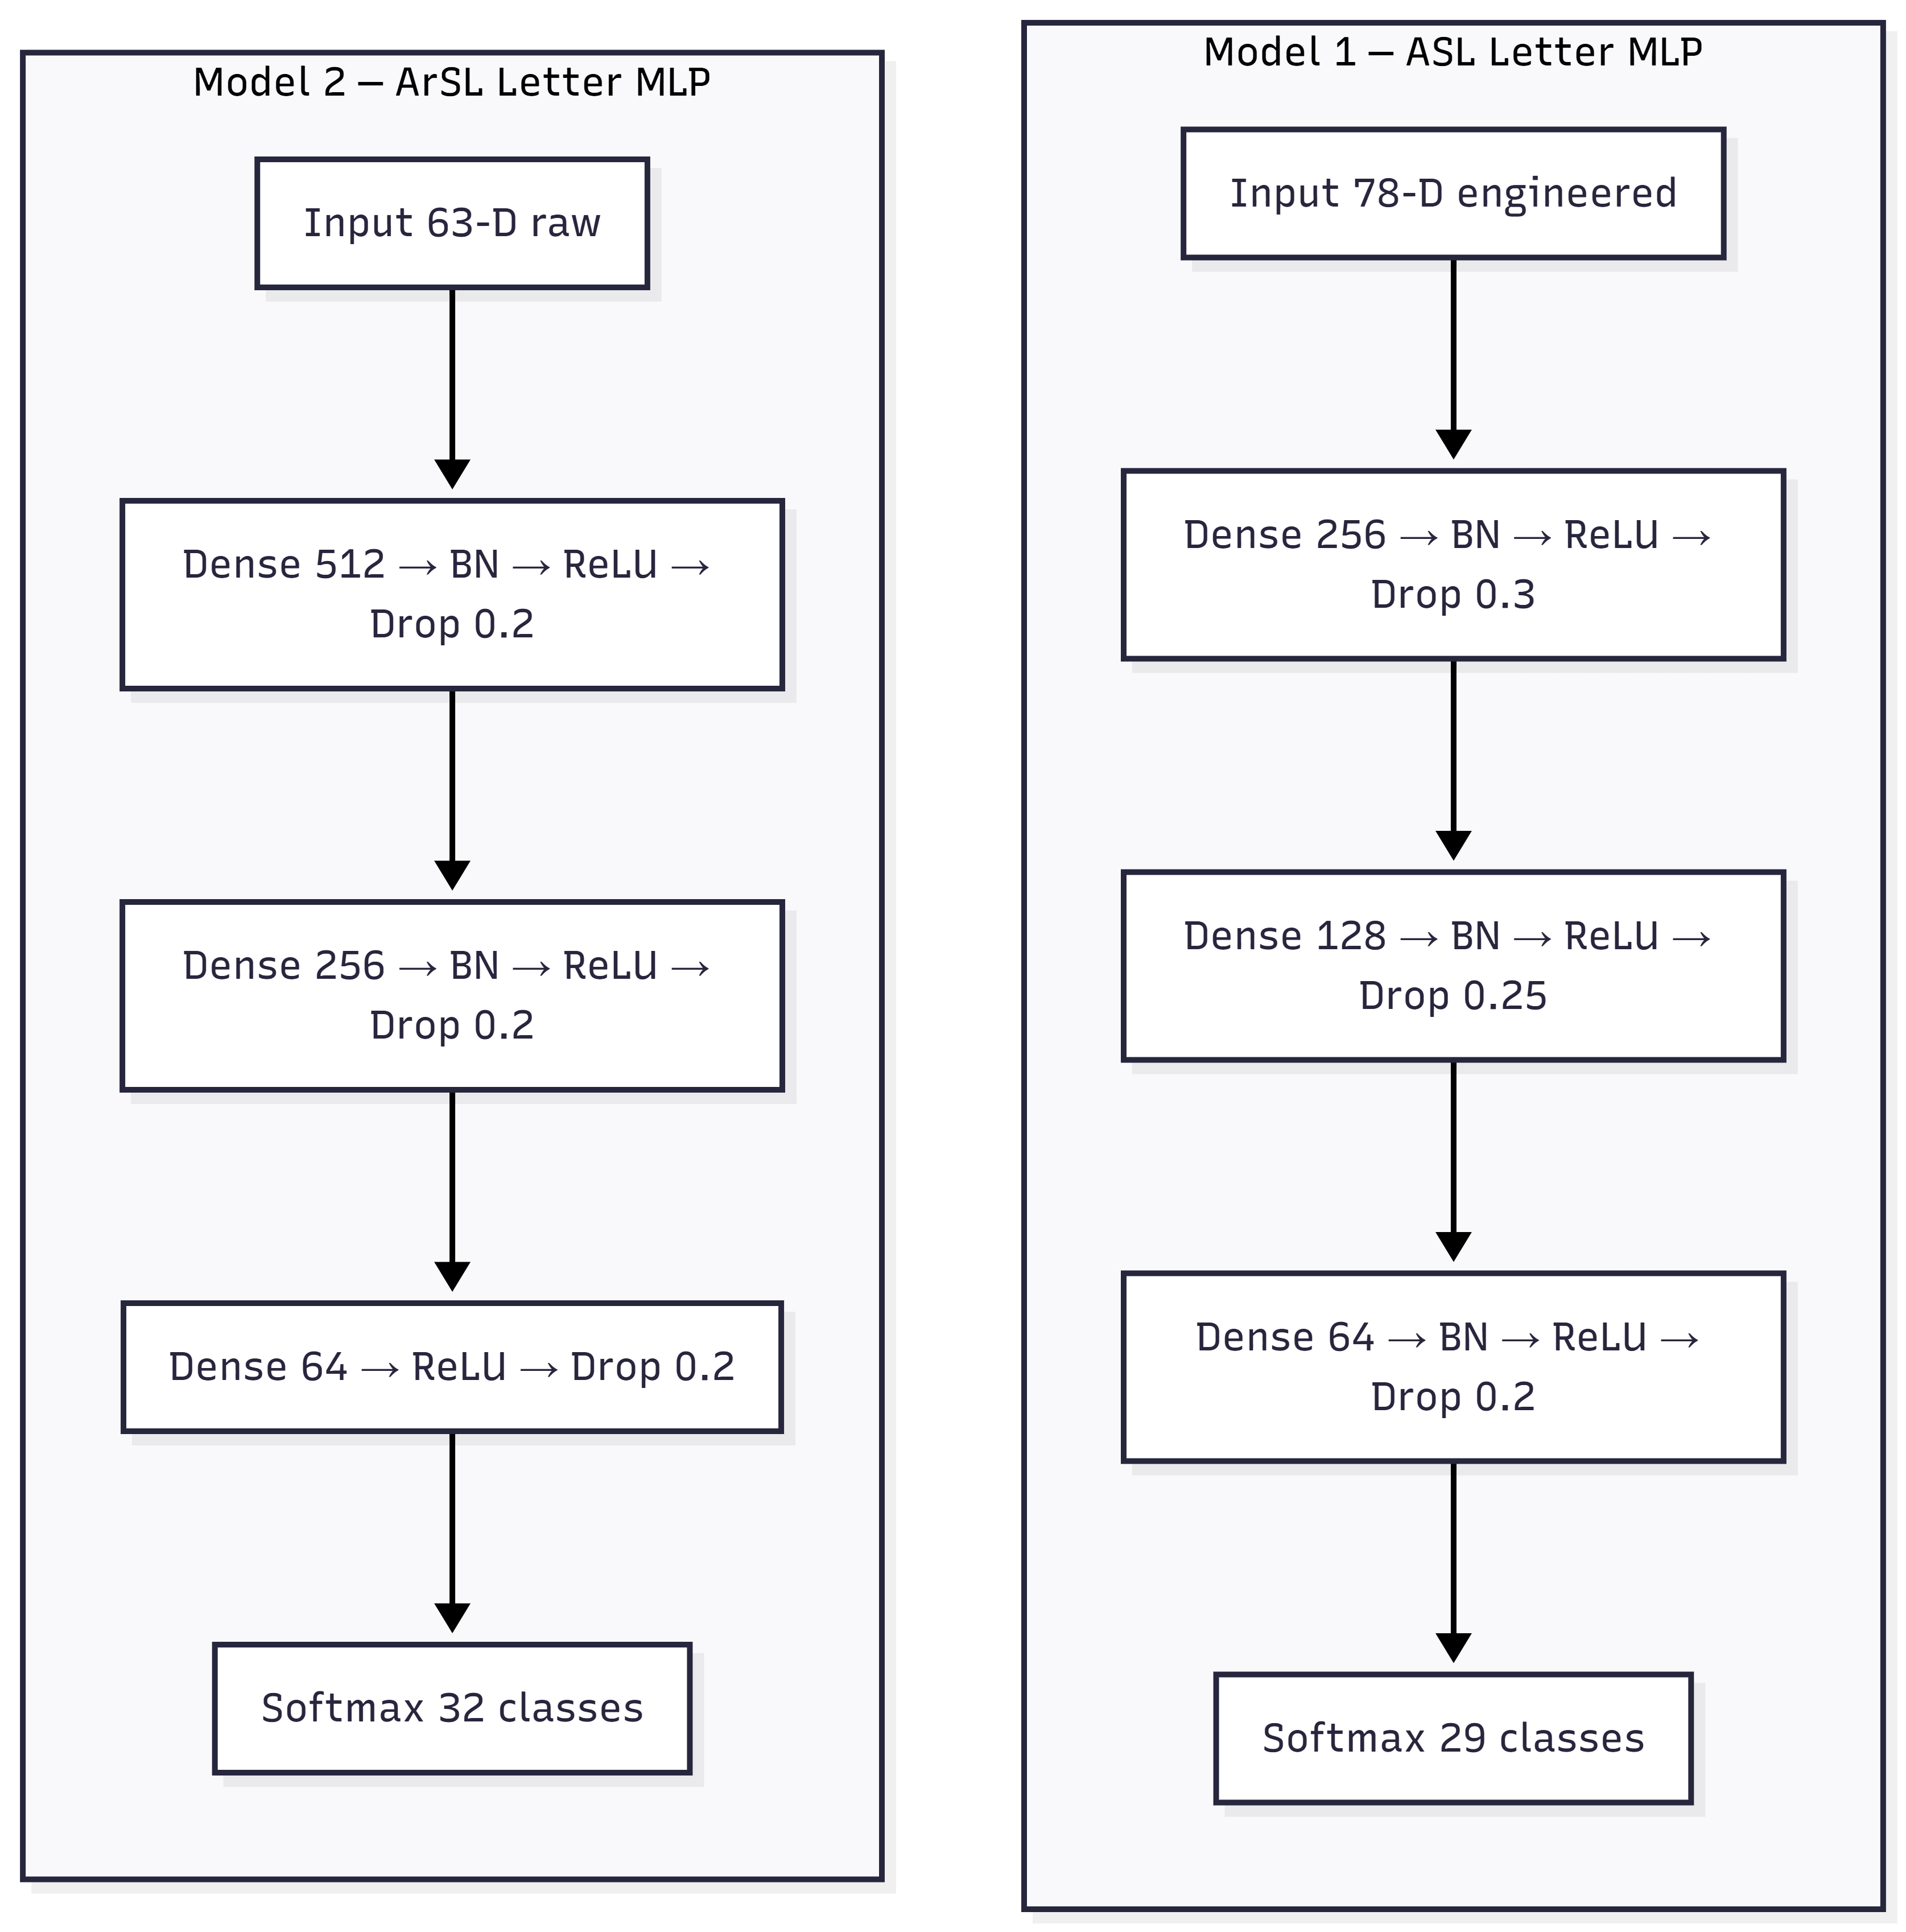
\includegraphics[width=0.88\textwidth]{images/fig_3-9_letter_mlp_heads.png}
\caption{Side-by-side comparison of the two letter MLP heads. Both follow Dense--BN--ReLU--Dropout blocks ending in softmax, but Model~2 uses a wider hidden stack (512/256/64), uniform dropout, and BN on layers~1--2 only.}
\label{fig:ch3-mlp-heads}
\end{figure}
\vspace{0.6cm}

% --- 3.6 STABILISATION ---
\noindent\textbf{3.6\quad LETTER STABILISATION DECODER}\par
\addcontentsline{toc}{section}{\numberline{3.6}LETTER STABILISATION DECODER}
\vspace{0.4cm}

\noindent Per-frame MLP outputs flicker under webcam noise. A finite-state stabilisation policy (as illustrated in Figure~\ref{fig:ch3-stabilisation}) buffers the last \textbf{10} frame labels, commits only when the buffer is full and the dominant label appears in at least \textbf{7 of 10} frames ($\geq$70\,\%), then enforces a \textbf{0.8\,s} hold before the next commit. \texttt{nothing} predictions clear the buffer; duplicate labels during the hold period are suppressed; a new label during hold resets the committed state. These thresholds match the deployed \texttt{letter\_\allowbreak stream\_\allowbreak decoder.py} logic in the FastAPI/React web stack (Chapter~6).\par\vspace{0.3cm}

\noindent A standalone desktop test setup used a stricter policy of 15 frames, 11-of-15 majority, and 1.2\,s hold; those parameters are retained for offline desktop testing but are not part of the web deployment.\par\vspace{0.4cm}

\begin{figure}[H]
\centering
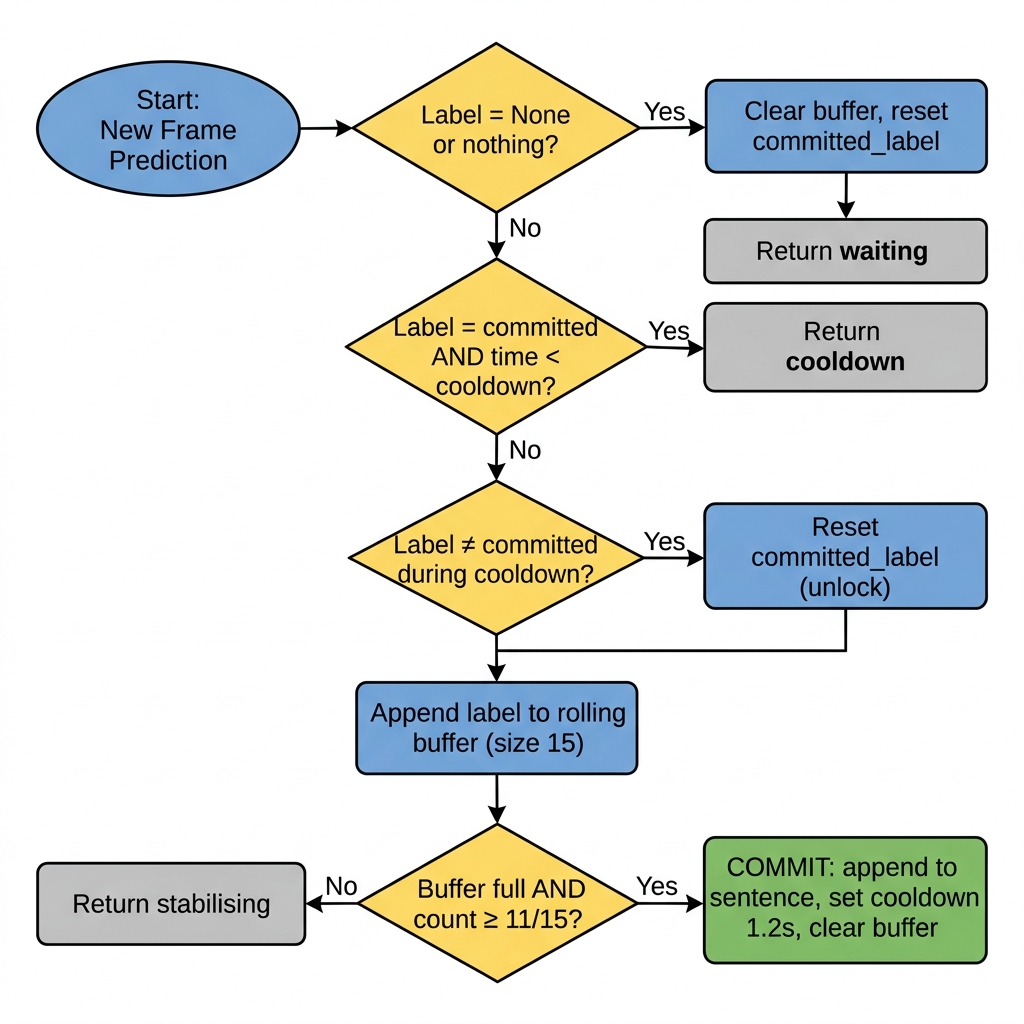
\includegraphics[width=0.75\textwidth]{images/fig_3-4_stabilisation_fsm.png}
\caption{Letter stabilisation finite-state machine. A rolling buffer of 10 frames requires $\geq$7 agreeing labels before \textbf{Commit}; a 0.8\,s hold prevents duplicate characters.}
\label{fig:ch3-stabilisation}
\end{figure}
\vspace{0.6cm}

% --- 3.7 ARABIC RENDERING ---
\noindent\textbf{3.7\quad ARABIC TEXT RENDERING}\par
\addcontentsline{toc}{section}{\numberline{3.7}ARABIC TEXT RENDERING}
\vspace{0.4cm}

\noindent ArSL letter labels are stored as romanised gloss strings (e.g.\ \texttt{bb}). Before display, the UI maps each gloss through \texttt{ARABIC\_MAP} to a Unicode glyph, applies \texttt{arabic\_reshaper}~\cite{arabicreshaper2024} for contextual form selection (isolated/initial/medial/final), reorders with \texttt{python-bidi}~\cite{pythonbidi2024,unicode2021bidirectional}, and renders with PIL/Pillow~\cite{pillow2024} using a TrueType Arabic font on the live HUD frame (as illustrated in Figure~\ref{fig:ch3-arabic-render}). English letter mode skips this pipeline and renders Latin glyphs directly.\par\vspace{0.4cm}

\begin{figure}[H]
\centering
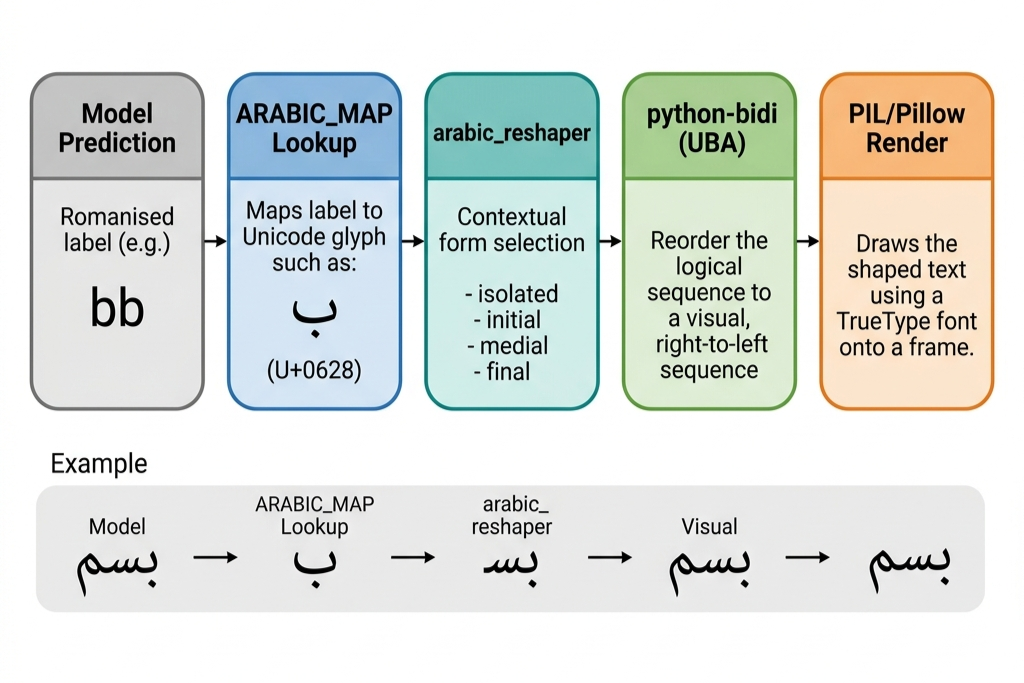
\includegraphics[width=0.9\textwidth]{images/fig_3-6_arabic_rendering.png}
\caption{Arabic UI rendering pipeline. Romanised model labels are mapped to Unicode, reshaped for cursive joining, reordered RTL with python-bidi, and drawn onto the webcam overlay (example: \texttt{bb} $\rightarrow$ ba glyph).}
\label{fig:ch3-arabic-render}
\end{figure}
\vspace{0.6cm}

% --- 3.8 TRADE-OFFS ---

\vspace*{-0.3cm} % Secret trick: Pulls the whole page's starting text slightly up into the top margin

\noindent\textbf{3.8\quad ENGINEERING TRADE-OFFS (LETTERS)}\par
\addcontentsline{toc}{section}{\numberline{3.8}ENGINEERING TRADE-OFFS (LETTERS)}
\vspace{0.2cm} % Cramped from 0.4cm

\begin{table}[H]
\centering
\caption{Engineering trade-offs for letter recognition in Eshara.}
\label{tab:ch3-tradeoffs}
\footnotesize % Shrunk from \small to save vertical space
\begin{tabular}{|p{0.26\textwidth}|p{0.30\textwidth}|p{0.36\textwidth}|}
\hline
\textbf{Decision} & \textbf{Alternative considered} & \textbf{Rationale} \\ \hline
Landmarks not pixels & MobileNetV2 on letter images & Webcam domain gap; unified live path \\ \hline
MLP for letters & BiLSTM per frame & No temporal signal; lower latency \\ \hline
63-D raw (ArSL) / 78-D (ASL) & Single shared feature size & ASL gains from angle features; ArSL stays lightweight \\ \hline
Wider ArSL MLP (512/256/64) & Same 256/128/64 stack as ASL & Higher intra-class variation; similar Arabic letter pairs \\ \hline
Stabilisation decoder & Raw per-frame display & Reduces flicker; improves UX \\ \hline
Web-only deploy & Mobile / TFLite & Graduation scope; WCAG browser access \\ \hline
\end{tabular}
\end{table}
\vspace{0.2cm} % Cramped from 0.6cm
\clearpage
% --- 3.9 EVAL ---
\noindent\textbf{3.9\quad EVALUATION PROTOCOL (LETTERS)}\par
\addcontentsline{toc}{section}{\numberline{3.9}EVALUATION PROTOCOL (LETTERS)}
\vspace{0.2cm} % Cramped from 0.4cm

\noindent Each letter model is evaluated on a \textbf{held-out test split} never used for hyperparameter tuning. Reported metrics (Chapter~6):
\vspace{-0.1cm} % Pulls the bulleted list closer to the sentence above it
\begin{itemize}
\setlength{\itemsep}{0pt} % Removes empty lines between bullet points
\setlength{\parskip}{0pt}
\item \textbf{Top-1 accuracy} --- both letter models.
\item \textbf{Confusion matrices} and per-class precision/recall --- error analysis (motion letters J/Z for ASL; visually similar pairs for ArSL).
\item \textbf{End-to-end latency} (ms) --- letter MLP path including stabilisation (Chapter~5, Section~5.12).
\end{itemize}
\vspace{0.2cm} % Cramped from 0.3cm

\noindent Chapter~4 describes word recognition methodology; Chapter~6 reports measured offline results; Chapter~5 describes the web implementation.\par\vspace{0.2cm}

\enlargethispage{2\baselineskip} % THE MAGIC BULLET: Forces LaTeX to make this specific page 2 lines taller at the bottom margin to catch any spilling text!

\noindent\textbf{Chapter summary.} Letter recognition in Eshara is implemented as two independent single-frame MLP classifiers behind one web API. Both share MediaPipe Hands extraction and the same offline training workflow (as summarised in Figure~\ref{fig:ch3-training-pipeline}), but ASL uses 78-D engineered features with a compact 256/128/64 head ($\sim$49\,k parameters), whereas ArSL uses 63-D raw features with a wider 512/256/64 head ($\sim$183\,k parameters) tuned for visually similar Arabic letter pairs (as compared in Figure~\ref{fig:ch3-mlp-heads} and Table~\ref{tab:ch3-arch-compare}). A stabilisation decoder suppresses per-frame flicker before the UI commits characters; Arabic output passes through a dedicated RTL rendering pipeline. Results for both letter models are reported in Chapter~6.\par

\clearpage